\chapter{Fundamentals} % Main chapter title
\label{chap:fund}

% Hier muss alles rein was benötigt wird um die Arbeit zu verstehen.
%   Man kann ja sicherlich grundlegendes Verständis von Recherstrukturen und Organisation vorraussetzten
%   Was also sollte definitiv nochmal erklärt werden?
%
%   - Virtual Memory -> Und vor allem die Kosten, das ist ja auch irgendwo der Aufhänger
%           Der Satz, "tlb is on the critical path of everything really" sollte irgendwann mal kommen
%   - Motivation für vm
%   - Organisationsstrukturen auch im vergleich -> Fazit: Page Tables sind überall und werden tiefer -> vor allem wegeb backwards compatiblity?
%   - Hardware Strukturen für VM - MMU, TLB
%   - Operating system and VM -> Implemented by OS but fixed structures given by MMU
%   -> Problem, fehlende flexibilität ->  A look at several ...
%   -> source: Architectural and operating system support for virtual memory
%   source: issues of implementation

% -------------------------------------------------------------------------------------------------
%                                           VIRTUAL MEMORY
% -------------------------------------------------------------------------------------------------

This chapter introduces some essential concepts and mechanisms which form the basis of the following
chapters. It first gives an overview of \textit{Virtual Memory (VM)}, its core requirements,
tradeoffs and implementations.
Then the hardware components and caches used to accelerate VM systems are
presented.
An overview of purely software-managed systems follows with a comparison of the general trade-offs
between software-managed and hardware-managed VM systems.
Finally, some specifics of the memory system of the chosen implementation platform, \textit{RISC-V},
are shown.

% Todo Overlaying
\section{Virtual Memory}
\textit{Virtual Memory} was first introduced in the Atlas System \cite{fotheringham1961dynamic} to
automate the task of swapping pages between main and secondary memory.
The idea was to make programs completely unaware of real, physical memory by providing
an abstraction layer called Virtual Memory \cite{denning1996virtual}.
With Virtual Memory, programs appear to have the whole memory space of the machine at their disposal. It also
hides the other processes and their memory from them.
The task of managing the memory of a program, no matter where in its virtual address space it is, and putting it somewhere
in physical memory now falls to the operating system \cite{denning1970virtual}.
This change to the operating systems role in managing program memory was not only useful but also necessary. The size of programs was increasing faster than the size of main
memory; while single programs
still fit in memory, operating systems make it possible to run multiple programs at once, collectively exceeding
the available physical memory \cite{tanenbaumOS}.
% -------------------------------------------------------------------------------------------------

\subsection{Virtual and physical addresses}
The terms of \textit{Virtual} and \textit{Physical} addresses are used a lot of this thesis.
Virtual addresses refer to those that are used by the program to reference a memory object in its address
space. They are only valid in the address space of the program. Thus, it is possible for programs to use the same
virtual addresses, which point to different physical addresses.
Virtual addresses are translated to physical addresses, which are actual addresses of memory. The \textit{VM System} is tasked with performing this translation, the creation of mappings,
and keeping track of those mappings \cite{denning1996virtual}.

Some memory systems which use inverted page tables also use the notion of \textit{effective} addresses.
These form an additional layer of indirection that allows the sharing of pages \cite{jacob1998virtualissues}.
Effective addresses will not be discussed here any further.
% -------------------------------------------------------------------------------------------------

\subsection{Memory System Requirements}
In modern systems, Virtual Memory does a lot more than swapping pages between main memory and secondary
storage and providing new pages of memory on-demand to programs.
It is the foundation of a number of requirements for the memory system that are taken for granted
\cite{jacobSoftwaremanagedAddressTranslation1997}.
These requirements are as follows:

% -------------------------------------------------------------------------------------------------

\paragraph{Address Space Protection / Isolation} It should not be possible for one process to access the data
of another process, unless explicitly shared.
\cite{jacobVirtualMemoryContemporary1998}

% -------------------------------------------------------------------------------------------------

\paragraph{Shared Memory} Sharing memory allows programs to work on the same physical data with potentially
differing virtual addresses \cite{jacobVirtualMemoryContemporary1998}.
Shared memory is used as a high-throughput mechanism for inter-process communication or for working on
a shared data structure \cite{tanenbaumOS}.

\begin{marginfigure}
    \includegraphics*[width=1\marginparwidth]{figures/fund_share.pdf}
    \caption{\textbf{Page Sharing} VM systems allow for the same physical page to be mapped into different virtual address spaces}
\end{marginfigure}

% -------------------------------------------------------------------------------------------------

\paragraph{Large Address Spaces} Programs tend to require more and more memory. Swapping memory can help
to support programs bigger than the actual size of main memory \cite{tanenbaumOS}, but programs may
also require more memory than the theoretical limit set by hardware and software. Modern architectures
use bigger addresses to support programs that require a lot of memory
\cite{jacobSoftwaremanagedAddressTranslation1997, jacobVirtualMemoryContemporary1998}.

% -------------------------------------------------------------------------------------------------

\paragraph{Fine-grained Protection} From a security perspective, it is often not desirable to e.g. allow the code segment
of a program to be writeable and the data section to be executable.VM systems provide read-only,
read-write and execute-only protection on a page granularity \cite{jacobSoftwaremanagedAddressTranslation1997}.
Illegal references may trigger exceptions, which allow the operating system to deal with the program \cite{jacobVirtualMemoryContemporary1998}.

% -------------------------------------------------------------------------------------------------

\paragraph{Superpages}
Structures may be bigger than a single page and may thus occupy multiple entries of the translation caches while
only referring to one object. To avoid displacing other caches entries, VM systems use
superpages to provide space for bigger objects to increase the reach of cache entries \cite{jacobSoftwaremanagedAddressTranslation1997}.

% -------------------------------------------------------------------------------------------------

\paragraph{Flexibility} Programmers should not have to think about the management
of the resources required to do their job, that is the job of the operating system \cite{tanenbaumOS}. As such, it should be possible to place code and data of the program anywhere in its virtual address space to make the programmer's
job as easy as possible and to increase the flexibility of the program
\cite{jacob1998virtualissues}. % Simplification of the programmes job

\begin{marginfigure}
    \includegraphics*[width=0.9\marginparwidth]{figures/fund_flexibility.pdf}
    \caption{\textbf{Flexibility} Program segments can be dispersed anywhere
        around the virtual address space; the VM system has to place
        the pages into actual physical memory.}
\end{marginfigure}
% -------------------------------------------------------------------------------------------------

\paragraph{Sparsity} Big addresses and fine granularity result in a huge address
space with a sparse population for programs that do not require a lot of pages
\cite{tanenbaumOS}.
A lot of programs do not require the full virtual address space and only occupy a small set of pages.
Bookkeeping of smaller address spaces should be as cheap as possible.

\begin{marginfigure}
    \centering
    \includegraphics*[width=0.5\marginparwidth]{figures/fund_sparsity.pdf}
    \caption{\textbf{Sparsity / Large Address Spaces} VM Systems need to efficiently
        realize huge address spaces with only a few pages being used.}
\end{marginfigure}

% -------------------------------------------------------------------------------------------------

There are different ways how memory systems implement these requirements.
The two most common implementations are based on hierarchical/multi-level/radix
\cite{jacob1998virtualissues,yaniv2016hash,tanenbaumOS} page tables and inverted page tables \cite{jacob1998look,jacob1998virtualissues}.
These implementations are summarized next.




% -------------------------------------------------------------------------------------------------
%                                IMPLEMENTATION OF VIRTUAL MEMORY
% -------------------------------------------------------------------------------------------------

% Wie können wir VM realisieren? -> Verschiedene Implementationen, Aber hier nicht auf die HW eingehen
%   [ A look at several...]
%   [ Issues of implementation]
\subsection{Implementation of Virtual Memory}
Every Virtual Memory system must realize a mapping from virtual addresses of each process-private virtual address space to physical addresses that index data in main memory.
This section will provide an overview of how the most commonly used VM implementations satisfy
this requirement.


% Naive approache
The naive approach is to simply have a big array in main memory. This array can be indexed
using the virtual addresses, at which the physical address to that virtual address is placed.
In a 32-bit address space with 4 KB pages, this requires 20 bits per page table entry. This
adds up to \[ 20 * 2^{20} bit = 20971520 / 8 Byte = 2.5 MB \]
To properly isolate the processes from each other, every process must have an array as outlined above.
Aditionally, each array should include additional bits for read/write/execute rights, in order to realize fine-grained protection of pages.
With a 64-bit computers, the space requirements for such page tables would be even higher.

% Hierarchical
\subsubsection{Hierarchical/radix/multi-level page tables}
To reduce the memory cost of managing pages, most \todo{cite?} VM systems use a
multi-level page table, also known as a hierarchical page table. However, its structure
is less like a table and more like a tree, in which the nodes are tables of page table entries (PTEs) \cite{tanenbaumOS}.
Here the virtual page number is divided into several parts. Each part of the Virtual Page Number (VPN)
is used to index a smaller table. The indexed PTE then points to the next smaller page table,
which in turn is indexed by the next part of the VPN. Depending on the implementation
this can involve up to 5 further indirections.
RISC-V, the architecture the implementation of this paper is based on, offers a 3-level page table
design \cite{riscvreader}.
The deconstruction of the virtual address and construction of the physical address of this
scheme is shown in \ref{fig:fund:pagetree}.
For bigger address space, RISC-V also offers 4 and 5-level schemes.

\begin{figure*}[t]
    \centering
    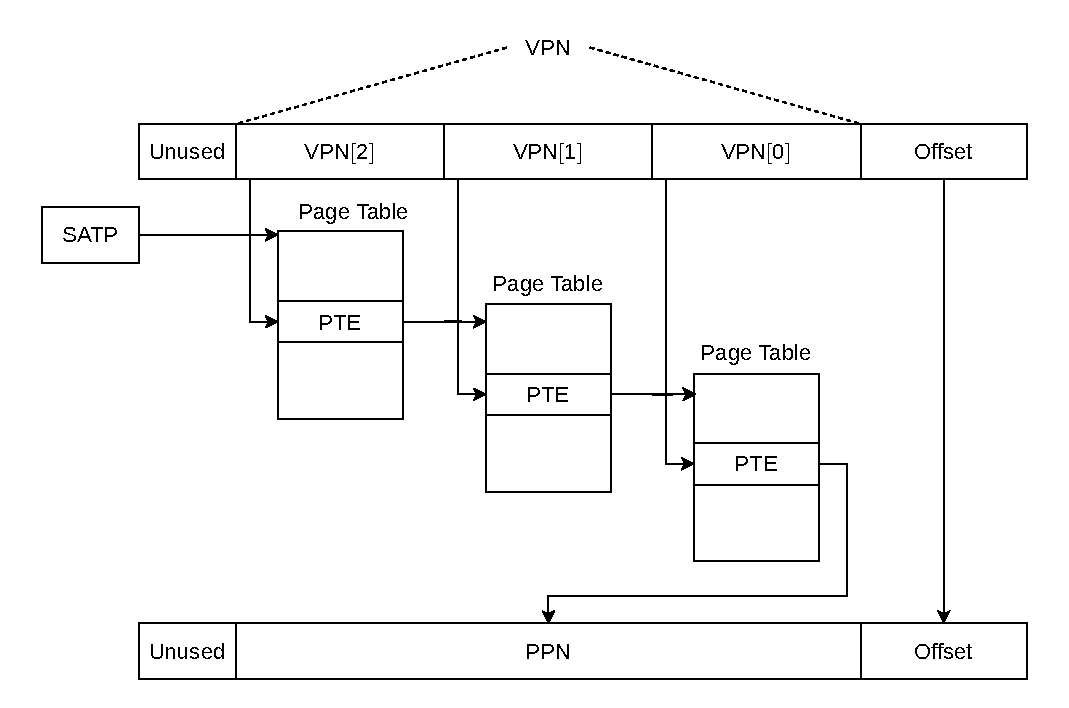
\includegraphics[scale=.8]{figures/VM-Tree.pdf}
    \caption[RISC-V Sv39 3-Level Page Tree]{Three-step page walk with a RISC-V Sv39 Page Table Tree:
        The value in the \texttt{satp} register is the base of the root page table; \texttt{VPN[2]}
        is the index into the root page table; the indexed \texttt{PTE} points to the next page table.
        This traversal continues until the bottom of the page table is reached (or until
        a valid PTE is found). The last \texttt{PTE}
        contains the \texttt{PPN} of the physical address which can then be combined with the offset
        bits to make the full physical address \cite{riscvreader}}
    \label{fig:fund:pagetree}
\end{figure*}


% Conclusion -> Many main memory accesses -> Expensive
Traversing the page table to find the mapping requires an additional memory reference for each
level \cite{jacobVirtualMemoryContemporary1998}, and since finding the mapping is on the critical path of every memory operation,
in the worst case, if all caches miss, up to 5 memory accesses may be required (in a 5-level paging
scheme) just to find the mapping for a single memory access.

% Solution? Hashed!
\subsubsection{Inverted page tables}
An alternative paging scheme approaches the problem from the opposite direction and provides a PTE
for each physical frame instead of one entry per virtual page.
A physical page frame is a page-aligned space in physical memory for a page.
The number of physical frames is determined by the size of main memory divided by the page size.
This has the enormous advantage that the bookkeeping only needs to keep record of as many pages
as the physical memory can support.
In contrast, hierarchical page tables need to keep track of as many pages as there can be in the virtual
address space of all processes combined. That is a huge memory overhead compared to inverted page tables
\cite{jacob1998look}.
The page table design also has the advantage that, in the best case, significantly fewer main memory
accesses are required. In the simple design shown in figure \ref{fig:fund:inverted}, the corresponding
page table entry can be found with just two memory lookups \cite{skarlatos2020elastic}.

\todo{this is a lot of text with no image an no emphasize/fat}
% How can it use so little memory
To get a deterministic mapping from virtual to physical address, \emph{Inverted Page Tables} are indexed
using a hash calculated from the VPN.
Since the domain of the hash functions (virtual address space) is much bigger than its codomain (physical page frames),
collisions can happen. These collisions are stored in a linked list. Since
the collision chains can potentially become infinitely long, the access time of the inverted page table is theoretically
unbounded \cite{tanenbaumOS}.

% Hierarchical -> fixed number of refs (but memory usage)
Hierarchical page tables have the key advantage that they always require
a fixed number of memory accesses to determine the PTE.

% Hash anchor to reduce the number of collisions
Typical inverted page table designs often include a so-called hash anchor table, which is then
indexed by the calculated hash. Entries in the hash anchor table point to entries in the inverted page table
containing the actual PTEs. If the hash anchor is twice the size
of the page table, the average collision chain length can be halved \cite{jacob1998virtualissues}.
However, at least one additional memory reference is required in any case \cite{jacob1998virtualissues}.
Alternative designs for inverted page tables allow the table to be dynamically resized to avoid hash collisions.
But resizing the whole page table is very expensive and should be avoided \cite{skarlatos2020elastic}.

% Inverted Page Table figure
\begin{figure*}[t]
    \centering
    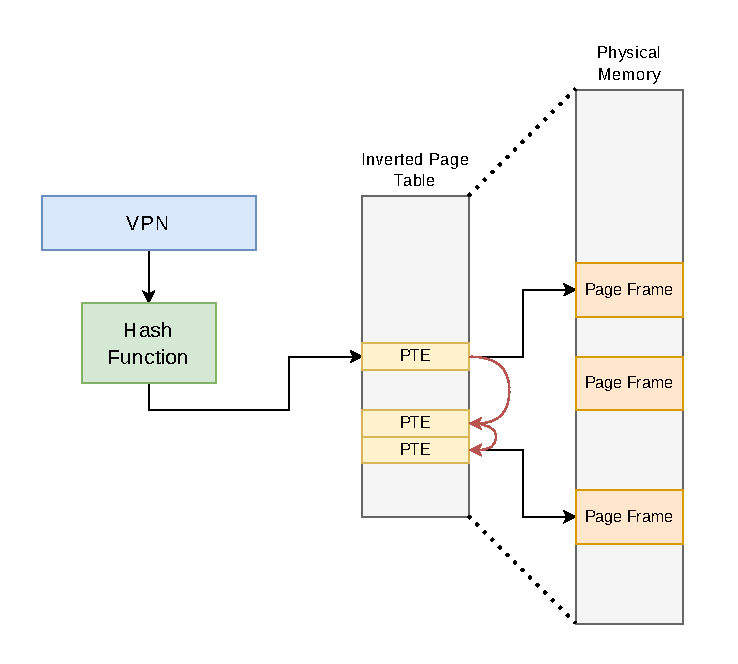
\includegraphics[scale=1]{figures/inverted_pt.pdf}
    \caption[Simple Inverted Page Table Design]{An inverted page table has an entry for every physical
        page frame, reducing memory accesses to a minimum of one. Collisions in the hash table (red arrows) can
        make the access much more expensive. }
    \label{fig:fund:inverted}
\end{figure*}


% Conclusion -> Disadvantages of inverted page tables [see also hash don’t cache!]
Inverted page tables significantly reduce the average access time to the PTEs, but they make it
more difficult to support other features like superpages and memory sharing.
The Power Architecture, for example, supports this through a two-stage translation process \cite{yaniv2016hash}.


% -> Most commonly used in today's hardware -> Multi level page tables
There is no clear winner in the debate between hashed and multi-level page tables.
Superiority of one design over the other also appears to depend on the computer architecture \cite{barrTranslationCachingSkip}
and the specific implementation of the design \cite{yaniv2016hash}.
Commercial hardware supports a variety of designs that are not standardized and, in some cases,
differ significantly \cite{jacob1998look}.

Modern Intel processors now support radix designs with a depth of up to 5 levels,
which still use 4KB pages to maintain compatibility.


% -------------------------------------------------------------------------------------------------
%                                  END SECTION - VM IMPLEMENTATION
% -------------------------------------------------------------------------------------------------



% -------------------------------------------------------------------------------------------------
%                                            VM HARDWARE
% -------------------------------------------------------------------------------------------------
\section{Memory Management Hardware}
To further accelerate the translation of virtual to physical addresses, most modern computers use additional
\cite{denning1970virtual} hardware components. These consist of a hardware page table walker (MMU) and a translation cache,
commonly referred to as a Translation Lookaside Buffer (TLB) \cite{jacobVirtualMemoryContemporary1998}.

% Frage: Besteht das MMU aus TLB + State Walker oder ist MMU der State Walker und TLB einfach extra?
% FIGURE Simple HW Architecture for VM Acceleration Hardware
\begin{figure*}[t]
    \centering
    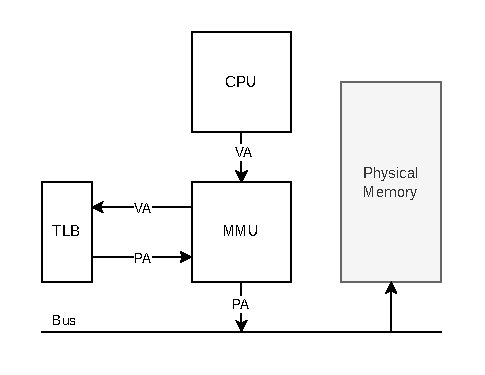
\includegraphics[scale=1.2]{figures/simple_mmu_arch.pdf}
    \caption[A simplified architecture of CPU, MMU and TLB]{A simplified architecture of CPU, MMU and TLB:
        User-level programs running on the \texttt{CPU} try to access main memory with virtual
        addresses; virtual addresses get transparently translated to physical addresses by the
        \texttt{MMU} by either looking up the address in the TLB or by performing a page table
        lookup with the hardware-supported page table design}
    \label{fig:fund:simplearch}
\end{figure*}
% End Figure

% -------------------------------------------------------------------------------------------------

\paragraph{MMU}
The Memory Management Unit (MMU) takes on the task of address translation for the computer.
It sits between the processor, which primarily works with virtual addresses, and the memory bus,
which is accessed with physical addresses. When the processor accesses a certain virtual address,
the MMU performs a page table walk to determine the physical address corresponding to the virtual
address. During this process, the processor is effectively frozen \cite{jacobVirtualMemoryContemporary1998}.

%TODO TLB as interface for VM

\paragraph{TLB} Since it would be very costly to traverse the page table in hardware for every load or store memory access, there is a cache for the translations, the Translation Lookaside Buffer (TLB). This cache contains the most recent translations from virtual to physical addresses. The MMU can first check the TLB, which can be searched in parallel and thus extremely quickly \cite{drepper2007every,jacobVirtualMemoryContemporary1998}.


% CONTINUE HERE!!!!!!!!!!!!!!!!!!!!!!!!!!!!!!!!!!!!!!!!!!!!!!!!!!!!!!!!!!!!!!!!!!!!!!!!!!!!!!!!


% -------------------------------------------------------------------------------------------------
\paragraph{Address Space Identifiers}
% \cite{jacobSoftwaremanagedAddressTranslation1997}
Address space identifiers (ASIDs) are number assigned to a process to identify pages associated with that process. This allows a more efficient use of the VM system: Normally, the TLB is flushed completely on context switch to avoid access to mappings from other processes. If ASIDs are used, only the mappings associated with the process leaving the CPU are flushed, leaving translations for globally valid mappings and shared pages in the TLB \cite{RISCVInstructionSet}.

\paragraph{SFENCE.VMA} RISC-V provides one instruction that acts primarily as a memory barrier:
It prevents reordering of instructions accessing memory accross the \texttt{sfence.vma} instruction.
This is important when the page tables are switched, e.g. when the kernel is entered from user mode,
because the translations will change.
The instruction also acts as a flushing operation for TLB entries. With both optional register
arguments set to zero, the instruction will flush all entries.
Setting the first register to a specific address will only flush translations containing that address.
The second register specifies the address space that is supposed to be flushed, given an ASID.

This mechanism allows for a precise control over the flushing of TLB entries, which can improve the
memory system performance \cite{RISCVInstructionSet}.



% -------------------------------------------------------------------------------------------------


% Fazit -> Es gibt hardware strukturen die VM beschleunigen können, die machen es auch schneller
%       ABER: Die machen die VM Software Systeme auch sehr viel rigider und unflexibler
% Kurze Diskussion -> Machen Hardware strukture das wirklich schneller? [ A look at ...]



% -------------------------------------------------------------------------------------------------

% -------------------------------------------------------------------------------------------------

\section{Software-based Virtual Memory System}
% VM in Software möglich mit ähnlicher Performance wie hw möglich -> Sollte ja mehr Flexibilität geben
%   [ A look at several...]
% Software managed address translation
% \subsection{Guarded Page Tables}

Software-based Virtual Memory Systems are generally more flexible than hardware-based systems
as the mapping can be controlled in software and structures (such as the PTE) are not bound
to the hardware \cite{jacob1998virtualissues}.
However, all of the approaches listed here still use a page table structure to keep track of mappings.
The main differences are in the details of the implemented page table structure and the way the software has to create the mappings. This freedom allows adjusting the VM system to fit more specific use cases, as hardware-based systems are designed to service a wide range of different applications \cite{jacob1998look}.
In the following, a number of software-based VM Systems are presented.
% A look at several
% MIPS -Ultrix
% Software managed tlbs
\subsection{MIPS}
MIPS \cite{MIPSArchitectureProgrammers2016} allows software-management of TLBs by raising an exception on TLB miss and by providing instructions to write TLB entries from software.
The Virtual Memory management systems \textit{Ultrix} and \textit{Guarded Page Tables} are implemented on top of MIPS.

\paragraph{Ultrix} The Ultrix page table is a two-tiered page table with two exception handlers for the TLB miss exception.
One of the handlers services user-level misses, the other one handles kernel-level misses.
Kernel level misses may occur when the page containing a PTE is not loaded and causes a
TLB miss \cite{jacob1998look}.

\paragraph{Guarded Page Tables} In his dissertation, Jochen Liedtke presented an innovative approach
to handling Virtual Memory\cite{liedtkeGPT}.
It is based on hierarchical page tables, and is shown to provide an efficient solution particularly in systems with large, sparse address spaces.
The design allows skipping over PTE entries to reach valid PTEs faster, without having to traverse every single level of the tree.
Gernot Heißer showcased an implementation of that design in \cite{heiserAnatomyHighPerformanceMicrokernel}.

% PA-RISCV VM System
\paragraph{PA-RISC}
PA-RISC uses an inverted page table design. Similar to Ultrix, the inverted page table is searched in the TLB miss handler when a TLB miss occurs.
The TLB miss handler calculates the hash from the virtual address to locate the head of the hash collision chain and then searches linearily through the chain to find the mapping \cite{jacob1998look}.

\paragraph{NOTLB}
A comparative study conducted by Jacob et al. \cite{jacob1998look} looks at a software-managed VM Design that uses no TLB at all.
The design uses a two-level page table structure like the ULTRIX/MIPS design and organizes its address space into disjunct segments.
Instead of a TLB miss handler, there is a Cache-Miss handler that services misses in the virtual L2 cache.
Similar to the Ultrix design, there are two handlers to handle nested cache misses.


% What was the paper about software managed chaches?








% -------------------------------------------------------------------------------------------------
% -------------------------------------------------------------------------------------------------
\section{Hardware Virtual Memory vs Software Virtual Memory}
% related work will then come in to discuss approaches close to my approach
% With only software ptw process would have to context switch to the kernel -> Very expensive
% With an MMU the processor essentially just freezes until the memory operation has completed
% \subsection{HW-Dependent PTE Structure} -> inflexibility

%elaboration on general costs of page table walks -> basically exactly what related
% work motivated their designs with
There are several considerations that should be taken into account when comparing hardware and
software-managed translations.

\paragraph{Fixed Paging Structures} In hardware-managed Virtual Memory, the structures for page tables
and page table entries are fixed by the microarchitecture. As a result, the operating system cannot tailor
memory management to its purposes and use case, and it is stuck with the fixed design.
This also complicates the portability of system software, as there is no standard for these memory management
structures. Despite there being no significant performance differences among the various designs,
there is no standardization \cite{jacob1998look}.

\paragraph{Pipeline Freezing / Flushing} On a TLB miss\todo{already defined?},
with a hardware-managed TLB, only the pipeline freezes (at least for instructions dependent on
the memory access). However, with a software-managed TLB, control is handed back to the operating system
via an exception, which notes that the required address is not in the TLB (TLB miss exception).
The jump back to the operating system causes a context switch, requiring the state of the current process
to be saved. During this, the reorder buffer is flushed, and the pipeline is heavily disrupted.
Switching to the kernel can also lead to further data and instruction misses in the long term
as the kernel entry likely overwrites some cache lines that the running process needed. \todo{Cite}

\paragraph{Complexity} Choosing between hardware and software Virtual Memory is choosing where to shift the complexity.
Systems that do only support software managed VM systems are simpler on the hardware side, because the burden of managing the memory is shifted to the software, which in turn will be more complex.
This goes in both directions \cite{jacob1998virtualissues}.

% Conclusion of HW vs SW
\cite{jacob1998look} concludes in a comparative study of various hardware and software memory designs
that hardware-based approaches are generally more performant, but software-based designs are certainly
viable if the caches are large enough to reduce the number of cache misses.
Especially in terms of flexibility, software-based approaches have a significant advantage,
as the VM system can be fully defined by the operating system.

% -------------------------------------------------------------------------------------------------

% -------------------------------------------------------------------------------------------------

% TODO Short discussion hw and sw vm -> common problem: Page Table Walks require in either case a
% lot of memory references. These costs can be aleviated using caches, but will still cost [ cite a source abouts costs here]

\todo{section on basic operating system structures like exception handler, load store sandwich}

% -------------------------------------------------------------------------------------------------

% -------------------------------------------------------------------------------------------------


\section{RISC-V Basics}
The implementation presented in this work runs on a RISC-V platform. Therefore, it is necessary
to go over some basic concepts of this platform. Particularly relevant here are the virtual
memory system, the exception/trap mechanism, and the control and status registers (CSRs), which
form the foundation for extending RISC-V.
The information presented in the following section is taken from both the RISC-V Reader \cite{riscvreader} and the RISC-V ISA Specification \cite{RISCVInstructionSet}.

% -------------------------------------------------------------------------------------------------

\subsection{Sv39 Virtual Memory}
\label{fund:sv39}

The RISC-V ISA specifies a simple, modular and scalable page-based VM system \cite{riscvreader}.
It supports different page sizes as well as different addressing modes:
Sv32 for 32-bit systems; Sv39 for 64-bit systems with a 3-level page table.
For bigger memory needs, there are the Sv48 and Sv57 addressing modes, adding one and two levels to the page table and supporting 256 TB and 128 PB respectively.
The following will only look at specifics for the Sv39 addressing mode.

The page table is an orthodox hierarchical multi-level page table, where each Page Table Entry (PTE) points to a PTE in the next level.
Each level of the page table contains 512 PTEs, 64-bit in size, bringing a page table to exactly 4 KB in size.
The format of a PTE is shown in figure \ref{fig:theory:sv39pte}.
\todo{explain why the top bits in PTE are all zero (with leichten Bezug zu xv6 impl)}
\begin{figure*}[h]
    \centering
    \begin{bytefield}[bitwidth=\widefigurewidth/64,bitheight=\widthof{~PBMT~}, bitformatting={\tiny\bfseries}, boxformatting={\centering}]{64}
        \bitheader[endianness=big]{63,62,61,60,54,53,28,27,19,18,10,9,8,7,6,5,4,3,2,1,0} \\
        \bitbox{1}{N} &
        \bitbox{2}{\rotatebox{90}{PBMT}} &
        \bitbox{7}{Reserved} &
        \bitbox{26}{PPN[2]} &
        \bitbox{9}{PPN[1]} &
        \bitbox{9}{PPN[0]} &
        \bitbox{2}{\rotatebox{90}{RSW}} &
        \bitbox{1}{D} &
        \bitbox{1}{A} &
        \bitbox{1}{G} &
        \bitbox{1}{U} &
        \bitbox{1}{X} &
        \bitbox{1}{W} &
        \bitbox{1}{R} &
        \bitbox{1}{V}
    \end{bytefield}
    \caption[RISC-V Sv39 Page Table Entry]{\textbf{RISC-V Sv39 Page Table Entry} }
    \label{fig:theory:sv39pte}
\end{figure*}

\todo{describe format}
The translation process (which was already shown in Figure \ref{fig:fund:pagetree}) splits the virtual address (See figure \ref{fig:theory:sv39va}) into 4 logical parts:
Three parts are parts of the Virtual Page Number (VPN), which are used to index the different page tables that are being traversed.
If the page table walk succeeds, the last PTE will contain a Physical Page Number (PPN), which will then be combined with the offset to create a physical address (See figure \ref{fig:theory:sv39pa}).


\begin{figure*}[h]
    \centering
    \begin{bytefield}[bitwidth=\widefigurewidth/56,bitheight=\widthof{~PBMT~}, bitformatting={\tiny\bfseries}, boxformatting={\centering}]{56}
        \bitheader[endianness=big]{55,30,29,21,20,12,11,0} \\
        \bitbox{26}{PPN[2]} &
        \bitbox{9}{PPN[1]} &
        \bitbox{9}{PPN[0]} &
        \bitbox{12}{Page Offset}
    \end{bytefield}
    \caption[RISC-V Sv39 Physical Address]{RISC-V Sv39 Physical Address}
    \label{fig:theory:sv39pa}
\end{figure*}

\begin{figure*}[h]
    \centering
    \begin{bytefield}[bitwidth=\widefigurewidth/39,bitheight=\widthof{~PBMT~}, bitformatting={\tiny\bfseries}, boxformatting={\centering}]{39}
        \bitheader[endianness=big]{38,30,29,21,20,12,11,0} \\
        \bitbox{9}{VPN[2]} &
        \bitbox{9}{VPN[1]} &
        \bitbox{9}{VPN[0]} &
        \bitbox{12}{Page Offset}
    \end{bytefield}
    \caption[RISC-V Sv39 Virtual Address]{RISC-V Sv39 Virtual Address}
    \label{fig:theory:sv39va}
\end{figure*}


Essential to the configuration of the VM system in RISC-V is the \texttt{satp} register (See figure \ref{fig:theory:sv39satp}).
It configures whether Virtual Memory is enabled at all or if direct mapping is used for all addresses. It is also used to set the addressing mode.
Beyond the configuration of the VM system, it contains the base address pointing to the root page table used for translations.

\begin{figure*}[t]
    \centering
    \begin{bytefield}[bitwidth=\widefigurewidth/64,bitheight=\widthof{~PBMT~}, bitformatting={\tiny\bfseries}, boxformatting={\centering}]{64}
        \bitheader[endianness=big]{63,60,59,44,43,0}\\
        \bitbox{4}{Mode} &
        \bitbox{16}{ASID} &
        \bitbox{44}{PPN}
    \end{bytefield}
    \caption[RISC-V Sv39 \texttt{satp} CSR]{RISC-V Sv39 \texttt{satp} CSR}
    \label{fig:theory:sv39satp}
\end{figure*}

% -------------------------------------------------------------------------------------------------

\subsection{Traps}
% exceptions vs interrupts
Traps are part of the RISC-V privileged architecture. They provide a mechanism to respond to
external events and unusual runtime events, known as exceptions \cite{riscvreader}.
The term "trap" is an umbrella term that is further divided into interrupts — asynchronous events —
and exceptions — synchronous events.
Exceptions are particularly of interest here, as a TLB miss occurs during the execution of an instruction,
meaning it happens synchronously with the processor's clock. However, it is important to keep interrupts
in mind when working with Qemu and xv6 source code, because the Qemu code handles exceptions
and interrupts within the same functions, and xv6, or RISC-V in general, uses a unified
vector for handling both interrupts and exceptions \cite{RISCVInstructionSet}.

% Exception registers
There are six central registers for triggering and handling exceptions. These exist both for
Supervisor Mode (prefixed with "s") and Machine Mode (prefixed with "m").
\todo{Have privilege modes been introduced already?}
Whether the machine mode or supervisor mode version of the register should be used for an exception depends
on the mode in which the exception is handled. In the following, all registers are presented with the
M-Mode prefix only. \todo{Has M-Mode as an abbreviation for Machine Mode been introduced?}
\todo{Because the exception was ultimately designed as an M-Mode exception?}

% TODO: sorting of registers by role?

% Vector -> mtvec
\paragraph{Exception Vector} The hardware thread (hart) \todo{Has the term "hart" been introduced?} experiencing
an exceptional state must know where the kernel routine is located to handle the exception.
The \texttt{BASE} field of the register contains a 4-byte aligned physical address to which
the program counter is set in the case of an exception.
The \texttt{MODE} field allows switching between \texttt{direct} and \texttt{vectored} modes.
In \texttt{MODE=Direct}, the PC is set to BASE for all traps, whereas in \texttt{MODE=Vectored},
the PC is set to $BASE+4*CAUSE$ for asynchronous interrupts.

% Delegation -> medeleg

% Data for exception handling -> mcause, mtval, mepc, mscratch
\paragraph{Context Information} To properly handle the exception, some context information is required.
The \texttt{mcause} register contains the exception code of the exception; \texttt{mepc} contains
the program counter of the instruction that triggered the exception; and \texttt{mtval} holds
exception-specific information, such as the virtual address that triggered a page fault exception.
\texttt{mstatus} contains general information about the current hardware state.

\paragraph{Delegation} Normally, all exceptions are handled in machine mode; however, in some cases,
it may be useful to handle the exception in a lower privilege mode. With the bitfield in the
\texttt{medeleg} register, individual exceptions can be chosen to be delegated to the next-lower
privilege mode.

% Exception number
\paragraph{Exception Code} Each exception is assigned a unique number, the exception code \cite{riscvreader}.
This can be found in the \texttt{mcause} register when handling the exception.


% Zusammenspiel der Register im Exception Fall -> xv6 Book Exception Machinery

\paragraph{Hardware Trap Mechanisms} When a trap is risen, the hardware does the following: \cite{cox2011xv6}
\begin{enumerate}
    \item interrupts are disabled by clearing the \texttt{MIE} bit i    \textbf{mstatus}
    \item \texttt{pc} is copied to \texttt{mepc}
    \item the current mode is saved to the \texttt{MPP} field in mstatus
    \item \texttt{mcause} is set to the proper exception code
    \item the mode is set to the machine mode
    \item \texttt{pc} is set to stvec
    \item execution continues at the new \texttt{pc}
\end{enumerate}
% -------------------------------------------------------------------------------------------------

\subsection{Control and Status Registers}
% Section describing RISC-V CSRs -> Originally in theory
The RISC-V ISA provides a 12-bit encoding space for 4096 CSRs. A CSR address is logically split
into four parts: The top two bits \texttt{csr[11:10]} specify whether the CSR is read/write or read-only;
\texttt{csr[9:8]} encode the minimum privilege level that is allowed to access the CSR; \texttt{csr[7:4]}
may be partially used to define a specific use for a range of CSRs. E.g. CSRs with an address
between \texttt{0x7B0} and \texttt{0x7BF} shall be used for Debug-mode-only CSRs \cite{RISCVInstructionSet}. The format
of the CSR addresses is also depicted in figure \ref{fig:theory:csr}.

% RISC-V CSR address bytefield
\begin{figure*}[h!]
    \centering
    \begin{bytefield}[bitwidth={2em}, bitformatting={\bfseries}, boxformatting={\centering}]{12}
        \bitheader[endianness=big]{11,10,9,8,7,4,3,0}\\
        \bitbox{2}{RW/RO} &
        \bitbox{2}{Priv} &
        \bitbox{4}{Usage} &
        \bitbox{4}{Index}
    \end{bytefield}
    \caption[RISC-V CSR address format]{\textbf{RISC-V CSR address format} \texttt{csr[11:10]} define whether the CSR is read-write or write-only; \texttt{csr[9:8]} defines the minimum privilege level that is allowed to access the CSR; \texttt{csr[7:4]} sets a directory within the CSR space for the usage of the CSR; \texttt{csr[3:0]} define an index}
    \label{fig:theory:csr}
\end{figure*}

Each legal CSR address identifies a CSR. The size of the CSRs identified by the CSR address depends
on the values of the SXLEN and UXLEN fields in the \texttt{mstatus} register. Currently, the
specification \cite{RISCVInstructionSet} allows for 32-bit, 64-bit and 128-bit.
% Short elaboration on using the csr to write TLB entries -> in the end its on the hardware implementor
RISC-V provides dedicated instructions for read/write and bit manipulation with both register values
and immediates.

% -------------------------------------------------------------------------------------------------






% All approaches are based on a table.
% Überleitung zu meinem Thema -> Avoid all memory references and just have a simple (hash?) function that realizes VM
% [ a look at severeal ] -> conlsion



